\documentclass[8pt]{beamer}
\usepackage[english]{babel}
\usepackage{pgf,graphicx}
\usepackage{amsmath,amssymb}
%\usepackage{bm}
\usepackage{stmaryrd}
%\usepackage[T1]{fontenc}
\usepackage[utf8]{inputenc}
%\usepackage{helvet}
%\usepackage{lmodern}
\usepackage{palatino}
%\usepackage{chancery}
\hypersetup{pdfpagemode = FullScreen,
						pdfauthor={Benjamin Steinert},
						pdftitle={SS 2018},
						pdfsubject={Presentation}}

%-----------------------------CI Farben deklarieren RGB-Format------------------------
\definecolor{orange}{rgb}{1.0,0.475,0}% RGB-Werte müssen normiert werden!(255=1.0)
\definecolor{black}{rgb}{0.00,0.00,0.00}
\definecolor{green}{rgb}{0,0.455,0.478}
\definecolor{blue}{rgb}{0,0.2,0.349}



%--------------------------------Hintergrundbild (CI TU-Ilmenau)--------------------------
\usepackage{eso-pic} % gutes Paket um Hintergründe einzufügen
\setbeamercolor{background canvas}{bg=} %beamer-eigenen Hintergrund Transparent setzten
\AddToShipoutPicture{ \put(0,0){%
     \parbox[b][\paperheight]{\paperwidth}{%
     \centering
     \rotatebox{0}{\includegraphics[width=1.0\paperwidth, height=1.0\paperheight]{bilder/Masterfolie.pdf}}
}}}

%---------------------------------Farben---------------------------------------------------
\setbeamercolor{structure}{fg=blue}%Farbe Inhaltsverzeichnis
\setbeamercolor{mini frame}{fg=orange}%Farben der aktiven Symbole in Navigationsleiste
\setbeamercolor{section in head/foot}{fg=orange}%Farbe der aktiven Abschnitte in Navigationsleiste
\setbeamertemplate{mini frame in other subsection}[default][10]%Sättigung der nicht-aktiven Symbole in Navigationsleiste
\setbeamertemplate{section in head/foot shaded}[default][10]%Sättigung der nicht-aktiven Abschnitte in Navigationsleiste
%\setbeamercolor{subsection in head/foot}{parent=palette primary}%Farbe Unterabschnitt in Navigationsleiste
\setbeamercolor{normal text}{fg=blue}%allgemeine Textfarbe
\setbeamercolor{title}{fg=blue}%Farbe Titel auf Titelbaltt
\setbeamercolor{item}{fg=green}%Farben für Blickfangpunkte (\itemize)

%------------------------------Seitenleiste und Fußleiste----------------------------------
\setbeamersize{sidebar width left=5mm}%Größe der linken sidebar

\setbeamertemplate{footline}{
  \leavevmode%
  \hbox{%
  \begin{beamercolorbox}[wd=0.95\paperwidth,ht=10ex,dp=8ex,left]{}%
     %\hspace{1cm} \insertsection
 	\hspace{0cm}\insertnavigation{0.6\paperwidth} %Navigationsleiste einfügen
  \end{beamercolorbox}% 
 \begin{beamercolorbox}[wd=0.05\paperwidth,ht=10ex,dp=8ex,center]{}%
  	%\insertsection
	\vspace{-5mm}%vertikale position dert Seitenzahlen
	\textcolor{white} {\insertframenumber / \inserttotalframenumber}%Seitenzahlen einfügen
  \end{beamercolorbox}}%
  \vskip0pt%
}


%--------------------------Allgemein------------------------------------------------------
\setbeamercovered{transparent}%Beamer-internes theme transparent schalten, um Hintergrundbild zu sehen
\usefonttheme{structurebold}
\beamertemplatenavigationsymbolsempty%Navigationshilfen an/aus
\newcommand{\stp}{\item[$\bullet$]}%\stp statt \item für Stichpunkt mit rundem Blickfangpunkt


%------------------------------------Titelseite-----------------------------------------------
\titlegraphic{\hskip5mm\includegraphics[width=3.5cm,height=0.8cm]{bilder/logo.pdf}}%Logo auf Titelseite 
\title{Is vagueness rational?}
\subtitle{Presentation of Bachelor-Thesis}
\author{Benjamin Steinert}
\institute[Eberhard Karls Universität Tübingen]{%
  Philosophische Fakultät\\
  Seminar für Sprachwissenschaft}
\date{11.06.2018}


%_____________________________________Slides___________________________________________________
\begin{document}

%______________________________________________________________________________________________
\frame{\titlepage}%Titelfolie
%______________________________________________________________________________________________

%______________________________________________________________________________________________
\section{Comic} 
\subsection*{}%Subsections nicht in Inhaltsverzeichnis (sonst ohne Stern)
\begin{frame}
\frametitle{Misinterpretation}
\vskip5mm
\hskip2cm
\includegraphics[scale=0.45]{bilder/misinterpretation.png}
(https://xkcd.com/1984/)
\end{frame}
%______________________________________________________________________________________________

%______________________________________________________________________________________________
\section{Problem statement} 
\subsection*{}%Subsections nicht in Inhaltsverzeichnis (sonst ohne Stern)
\begin{frame}
\frametitle{Problem Statement}
\vskip5mm
	\begin{itemize}
		 \stp Why is language vague?\newline
		 \stp Which processes enable us to understand vague adjectives like \textit{tall}?\newline
      	 \stp What is the exact semantics of such vague terms?\newline
      	 \stp Is vagueness rational?\newline
     \end{itemize}
\end{frame}
%______________________________________________________________________________________________

%______________________________________________________________________________________________
\section{Table of contents}
\frame{\frametitle{Contents}\tableofcontents[part=1]}%Folie mit Inhaltsverzeichnis
\part{Main Part}
%______________________________________________________________________________________________

%______________________________________________________________________________________________
\section{Pragmatics and Game Theory} 
\subsection*{}%Subsections nicht in Inhaltsverzeichnis (sonst ohne Stern)
\begin{frame}
\frametitle{Pragmatics and Game Theory}
\vskip5mm
	\begin{itemize}
        \stp \textbf{Pragmatics} is a subfield of linguistics.\newline
		\stp \textbf{(Evolutionary) Game theory} analyzes strategic interaction between individuals/agents.\newline
		\stp An \textbf{evolutionary stable strategy} cannot be further improved by other strategies in a population.\newline
     \end{itemize}
\end{frame}
%______________________________________________________________________________________________

%______________________________________________________________________________________________
\begin{frame}
\frametitle{Adjectival vagueness in language use}
\vskip5mm
Characteristics of vague adjectives:\\
\vskip5mm
	\begin{itemize}
		\stp Existence of \textbf{borderline cases}.\newline
		\stp \textbf{Threshold} semantics.\newline
    \end{itemize}
\end{frame}
%______________________________________________________________________________________________

%______________________________________________________________________________________________
\begin{frame}
\frametitle{Schematic presentation of crisp and vague denotations}

	\begin{columns}
		\column{7.8cm}
		\vskip5mm
		\includegraphics[width=7.8cm]{bilder/schema-crisp-vague.png}\\
		\vskip5mm
    	\column{4cm}
      	%\vspace{-1cm}
      	\begin{align*}
      	\rightarrow P(x \text{ is tall}) &= \Phi(P(\theta)) \\
		&= \llbracket \textit{"tall"} \rrbracket^x
      	\end{align*}
		\vskip3cm
		$\rightarrow P(\theta)$
	\end{columns}
\end{frame}
%______________________________________________________________________________________________

%______________________________________________________________________________________________
\section{RSA - Model}
\subsection*{}
\begin{frame}
\frametitle{RSA - Model}
\vskip5mm
	\begin{itemize}
		\stp The \textbf{rational speech acts model} (RSA model) is a cognitive model of language-understanding and -production.\newline
		\stp \textbf{Bayes' theorem: } $P(A \mid B) \propto P(B \mid A) \cdot P(A)$.\newline
		\stp An \textbf{informative speaker} chooses utterances, depending on their \textbf{informativity} for a hypothetical \textbf{literal listener}.\newline
		\stp A \textbf{pragmatic listener} infers world states (given a message) by reasoning about the speaker model and taking into account alternative messages. 
	\end{itemize}
\end{frame}
%______________________________________________________________________________________________

%______________________________________________________________________________________________
\begin{frame}
\frametitle{Extension to RSA by Bergen \& Goodman (2012)}
\vskip5mm
Agents are defined by \textbf{types}, that represent the semantic understanding:
\vskip5mm
	\begin{itemize}
		\stp \textbf{Literal listener}:\\
		$P_{L0}(w \mid m , \boldsymbol{ \big[ \mu, \sigma, \alpha\big]}) = \llbracket m \rrbracket^{w, \boldsymbol{ \mu,\sigma}} \cdot Pr(w) $\newline
		\stp \textbf{Informative speaker}:\\
		$P_{S1}(m \mid w, \boldsymbol{ \big[ \mu, \sigma, \alpha\big]}) \propto exp(\alpha \cdot log(P_{L0}(w \mid m, \boldsymbol{ \big[ \mu, \sigma, \alpha\big] })))$\newline
		\stp \textbf{Pragmatic listener}:\\
		$P_{L_1}(w \mid m, \boldsymbol{ \big[ \mu, \sigma, \alpha\big]}) \propto P_{S_1}(m \mid w, \boldsymbol{ \big[ \mu, \sigma, \alpha\big]}) \cdot Pr(w)$:
	\end{itemize}
\vskip5mm
\begin{align*}
\text{With: } w &= \text{world state (e.g. height),}\\
m &= \text{message,}\\
Pr &= \text{Prior,} \\
\mu, \sigma &= \text{Threshold parameters,}\\
\alpha &= \text{"Rationality" parameter}
\end{align*}
\end{frame}
%______________________________________________________________________________________________

%______________________________________________________________________________________________
\begin{frame}
\frametitle{Implementation of vagueness}
Literal vague meaning of \textit{tall} and \textit{not-tall}:
\vskip5mm
\includegraphics[width=9cm]{bilder/lit_tall_vague.pdf}
\end{frame}
%______________________________________________________________________________________________

%______________________________________________________________________________________________
\begin{frame}
\frametitle{Literal listener $L_0$ - Posterior}
$P_{L0}(w \mid m , \big[ \mu, \sigma, \alpha\big]) = \llbracket m \rrbracket^{w,\mu,\sigma} \cdot Pr(w) $:
\vskip5mm
\includegraphics[width=11cm]{bilder/L0-posterior.png}
\end{frame}
%______________________________________________________________________________________________

%______________________________________________________________________________________________
\begin{frame}
\frametitle{Informative speaker $S_1$ - Posterior}
\vskip5mm
$P_{S1}(m \mid w, \big[ \mu, \sigma, \alpha\big]) \propto exp(\alpha \cdot log(P_{L0}(w \mid m, \big[ \mu, \sigma, \alpha\big])))$:
\vskip5mm
\includegraphics[width=8.5cm]{bilder/S1-posterior.png}
\end{frame}
%______________________________________________________________________________________________

%______________________________________________________________________________________________
\begin{frame}
\frametitle{Pragmatic listener $L_1$ - Posterior}
\vskip5mm
$P_{L_1}(w \mid m, \big[ \mu, \sigma, \alpha\big]) \propto P_{S_1}(m \mid w, \big[ \mu, \sigma, \alpha\big]) \cdot Pr(w)$:
\vskip5mm
\includegraphics[width=7cm]{bilder/L1-posterior.png}
\end{frame}
%______________________________________________________________________________________________

%______________________________________________________________________________________________
\section{Simulation}
\begin{frame}
\frametitle{Goal of simulation}
\vskip5mm
	\begin{itemize}
		\stp Agents behave according to RSA.\newline
		\stp Examine effect of different semantic beliefs.\newline
		\stp Find out best strategy.\newline
	\end{itemize}
\includegraphics[width=13cm]{bilder/procedure.png}\\
\end{frame}
%______________________________________________________________________________________________

%______________________________________________________________________________________________
\begin{frame}
\frametitle{Measure of communicative success: Expected Utility}
The \textbf{Expected Utility (EU)} is calculated as followed:
\vskip5mm
\begin{align*}
EU(t_1, t_2) = \sum \limits_{w} \sum \limits_{m} 0.5 \cdot \big[ &P_{S_1}(m\,|\,w ,\, t_1) \cdot P_{L_1}(w \mid m ,\, t_2) \cdot Pr(w) + \\
&P_{S_1}(m \mid w ,\, t_2) \cdot P_{L_1}(w \mid m ,\, t_1) \cdot Pr(w) \big] \nonumber
\end{align*}
\end{frame}
%______________________________________________________________________________________________

%______________________________________________________________________________________________
\begin{frame}
\frametitle{Simulation set-up}
In the simulation, the types are combined from the following parameter spaces:
\vskip5mm
\begin{align*}
\mu &\sim \{ 0, 0.1, 0.2, ... , 1.9 \} \\
\sigma &\sim \{ 0.001, 0.1, 0.2, ... , 1.9 \} \\
\alpha &\sim \{ 1, 5, 10, 50, 100 \}\\
\\
M &= \{ short, not-short, tall, not-tall\}
\end{align*}
\end{frame}
%______________________________________________________________________________________________

%______________________________________________________________________________________________
\section{Simulation Results}
\subsection*{}
\begin{frame}
\frametitle{Simulation Results / EU data}
\vskip5mm
The \textbf{Expected Utility} values are displayed in a \textbf{heatmap} visualization.
Color-key-mapping:
\vskip5mm
\hskip2cm
\includegraphics[width=5cm]{bilder/color-key-mapping.png}

\end{frame}
%______________________________________________________________________________________________

%______________________________________________________________________________________________
\begin{frame}
\frametitle{Effect of parameter $\alpha$}
\vskip5mm
\hskip1cm
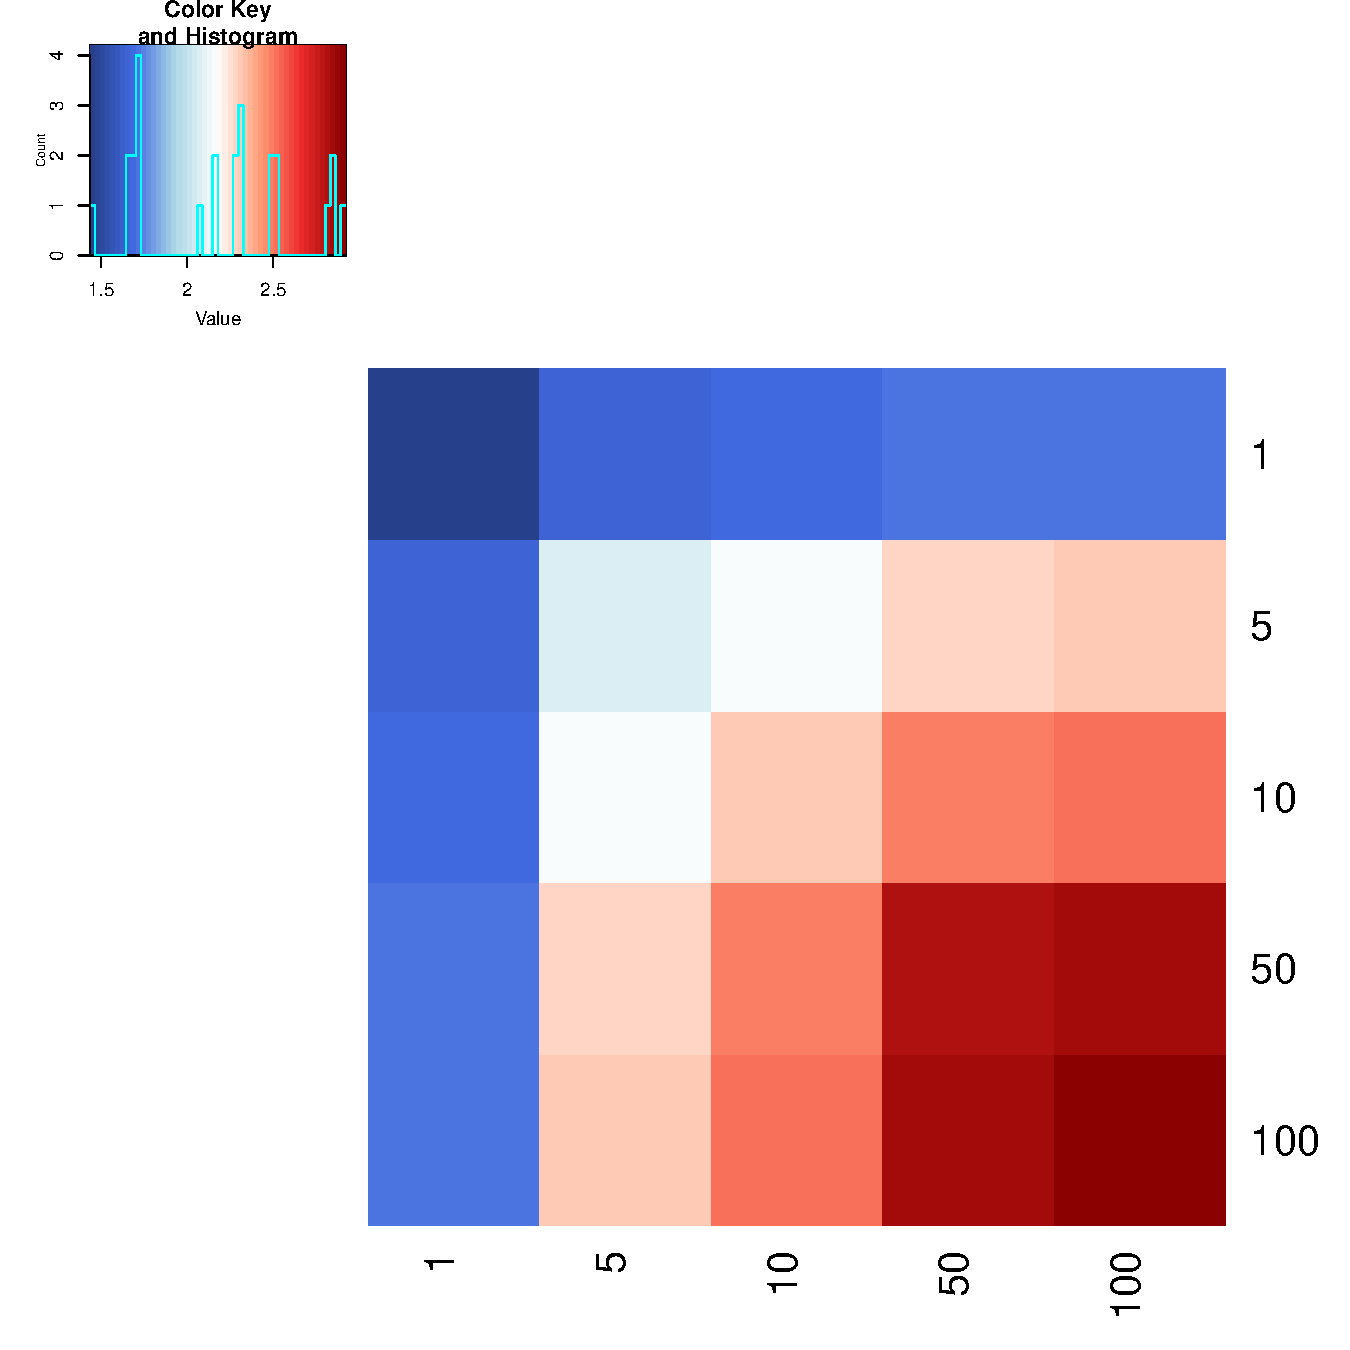
\includegraphics[width=7cm]{bilder/alpha_marg.pdf}
\end{frame}
%______________________________________________________________________________________________

%______________________________________________________________________________________________
\begin{frame}
\frametitle{Effect of parameter $\mu$}
\vskip5mm
\hskip1cm
\includegraphics[width=7cm]{bilder/mean_marg.pdf}
\end{frame}
%______________________________________________________________________________________________

%______________________________________________________________________________________________
\begin{frame}
\frametitle{Effect of parameter $\sigma$}
\vskip5mm
\hskip1cm
\includegraphics[width=7cm]{bilder/sigma_marg.pdf}
\end{frame}
%______________________________________________________________________________________________

%______________________________________________________________________________________________
\begin{frame}
\frametitle{Interaction effect of parameters $\alpha$ and $\sigma$}
\vskip5mm
\includegraphics[width=10.5cm]{bilder/EU-interaction-effect.png}
\end{frame}
%______________________________________________________________________________________________

%______________________________________________________________________________________________
\begin{frame}
\frametitle{Evolutionary stable strategies}
With $S$ = set of possible strategies.\\

Strategy $s_i$ is an ESS, if for all $s_j \neq s_i \in  S$:
\begin{align*}
1. EU(s_i, s_i) &\geq EU(s_j, s_i) \quad \textbf{and} \\
2. EU(s_i, s_j) &> EU(s_j, s_j)
\end{align*}
\vskip5mm
The only ESS is:\\
\vskip5mm
$type_{opt} = \big[ \mu=0.8, \sigma=0.5, \alpha=100 \big] $
\end{frame}
%______________________________________________________________________________________________


%______________________________________________________________________________________________
\section{Discussion}
\subsection*{}
\begin{frame}
\frametitle{Discussion and Conclusion}
\vskip5mm
	\begin{itemize}
		\stp Pragmatic recursive reasoning allows for interpretation of vague adjectives.\newline
		\stp Rational agents can make use of vagueness.  \newline
		\stp Vagueness indeed seems to be rational.\newline
	\end{itemize}
\end{frame}
%______________________________________________________________________________________________

%______________________________________________________________________________________________
\begin{frame}   % Vielen Dank
\frametitle{}
\vskip5mm
\begin{columns}
    \column{12cm}
 	\centering
	\huge{Thank you!}
 \end{columns}
\end{frame}
%______________________________________________________________________________________________


\end{document}


